\documentclass{article}
\usepackage{amsmath,amssymb}
\usepackage{mathtools}
\usepackage{amsfonts}
\usepackage{amssymb}
\usepackage{tikz}

\DeclarePairedDelimiter{\ceil}{\lceil}{\rceil}
\newcounter{question}
\setcounter{question}{0}
\begin{document}

\newcommand\Que[1]{%
   \leavevmode\par
   \stepcounter{question}
   \noindent
   \thequestion. Q --- #1\par}

\newcommand\Ans[2][]{%
    \leavevmode\par\noindent
   {\leftskip37pt
    A --- \textbf{#1}#2\par}}

\Que{  
  Perform the algorithm described in Theorem 5.13 on the graph in 
  Exercise 8. Make sure you do not try to be smarter than the algorithm, 
  in particular the following sentence followed exactly: 
  \textit{``We then choose the least integer $i$ for which there is an edge 
  incident with $x_i$ that has not already been traversed.''}\\

  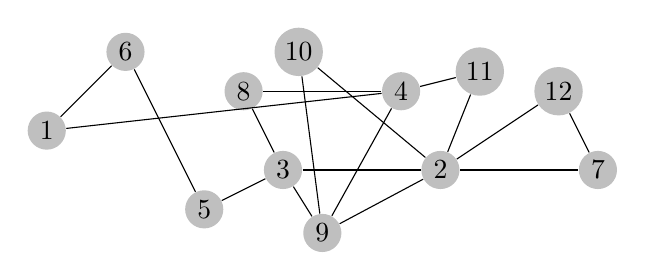
\begin{tikzpicture}[shorten >=1pt,->]
    \tikzstyle{vertex}=[circle,fill=black!25,minimum size=12pt,inner sep=2pt]
    \node[vertex] (G_1) at (0,0) {1};
    \node[vertex] (G_6) at (1,1) {6};
    \node[vertex] (G_5) at (2,-1) {5};
    \node[vertex] (G_3) at (3,-0.5) {3};
    \node[vertex] (G_8) at (2.5,0.5) {8};
    \node[vertex] (G_9) at (3.5,-1.3) {9};
    \node[vertex] (G_10) at (3.2,1) {10};
    \node[vertex] (G_4) at (4.5,0.5) {4};
    \node[vertex] (G_11) at (5.5,0.75) {11};
    \node[vertex] (G_2) at (5,-0.5) {2};
    \node[vertex] (G_7) at (7,-0.5) {7};
    \node[vertex] (G_12) at (6.5,0.5) {12};
    \draw (G_1) -- (G_6) -- cycle;
    \draw (G_1) -- (G_4) -- cycle;
    \draw (G_6) -- (G_5) -- cycle;
    \draw (G_5) -- (G_3) -- cycle;
    \draw (G_3) -- (G_8) -- cycle;
    \draw (G_3) -- (G_2) -- cycle;
    \draw (G_3) -- (G_9) -- cycle;
    \draw (G_8) -- (G_4) -- cycle;
    \draw (G_9) -- (G_4) -- cycle;
    \draw (G_9) -- (G_10) -- cycle;
    \draw (G_9) -- (G_2) -- cycle;
    \draw (G_10) -- (G_2) -- cycle;
    \draw (G_2) -- (G_11) -- cycle;
    \draw (G_4) -- (G_11) -- cycle;
    \draw (G_2) -- (G_7) -- cycle;
    \draw (G_2) -- (G_12) -- cycle;
    \draw (G_7) -- (G_12) -- cycle;
  \end{tikzpicture}\\
  }
\Ans{
  Eulerian algorithm:\\

  1) Starting with $(1)$, visit every connected vertex, 
  in the ascending order of ordinal until you reach $(1)$: \\

  $\textcolor{blue}{(1,4,8,3,2,7,12,2,9,3,5,6,1)}$\\

  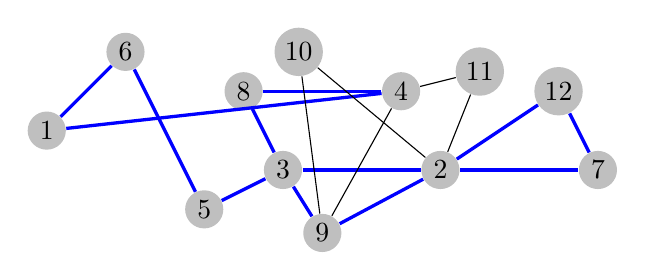
\begin{tikzpicture}[shorten >=1pt,->]
    \tikzstyle{vertex}=[circle,fill=black!25,minimum size=12pt,inner sep=2pt]
    \node[vertex] (G_1) at (0,0) {1};
    \node[vertex] (G_6) at (1,1) {6};
    \node[vertex] (G_5) at (2,-1) {5};
    \node[vertex] (G_3) at (3,-0.5) {3};
    \node[vertex] (G_8) at (2.5,0.5) {8};
    \node[vertex] (G_9) at (3.5,-1.3) {9};
    \node[vertex] (G_10) at (3.2,1) {10};
    \node[vertex] (G_4) at (4.5,0.5) {4};
    \node[vertex] (G_11) at (5.5,0.75) {11};
    \node[vertex] (G_2) at (5,-0.5) {2};
    \node[vertex] (G_7) at (7,-0.5) {7};
    \node[vertex] (G_12) at (6.5,0.5) {12};
    \draw [blue, very thick] (G_1) -- (G_6) -- cycle;
    \draw [blue, very thick] (G_1) -- (G_4) -- cycle;
    \draw [blue, very thick] (G_6) -- (G_5) -- cycle;
    \draw [blue, very thick] (G_5) -- (G_3) -- cycle;
    \draw [blue, very thick] (G_3) -- (G_8) -- cycle;
    \draw [blue, very thick] (G_3) -- (G_9) -- cycle;
    \draw [blue, very thick] (G_3) -- (G_2) -- cycle;
    \draw [blue, very thick] (G_8) -- (G_4) -- cycle;
    \draw (G_9) -- (G_4) -- cycle;
    \draw (G_9) -- (G_10) -- cycle;
    \draw [blue, very thick] (G_9) -- (G_2) -- cycle;
    \draw (G_10) -- (G_2) -- cycle;
    \draw (G_2) -- (G_11) -- cycle;
    \draw (G_4) -- (G_11) -- cycle;
    \draw [blue, very thick] (G_2) -- (G_7) -- cycle;
    \draw [blue, very thick] (G_2) -- (G_12) -- cycle;
    \draw [blue, very thick] (G_7) -- (G_12) -- cycle;
  \end{tikzpicture}\\

  2) If there are still unvisited edges,
  break the circuit at the lowest vertex incident with
  an unvisited edge: in this case, $(2)$ 
  and find a circuit using step $1)$ 
  back to this new starting point $(2)$: \\

  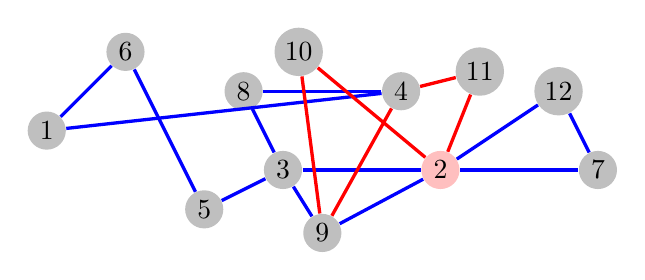
\begin{tikzpicture}[shorten >=1pt,->]
    \tikzstyle{vertex}=[circle,fill=black!25,minimum size=12pt,inner sep=2pt]
    \tikzstyle{redo vertex}=[circle,fill=red!25,minimum size=12pt,inner sep=2pt]
    \node[vertex] (G_1) at (0,0) {1};
    \node[vertex] (G_6) at (1,1) {6};
    \node[vertex] (G_5) at (2,-1) {5};
    \node[vertex] (G_3) at (3,-0.5) {3};
    \node[vertex] (G_8) at (2.5,0.5) {8};
    \node[vertex] (G_9) at (3.5,-1.3) {9};
    \node[vertex] (G_10) at (3.2,1) {10};
    \node[vertex] (G_4) at (4.5,0.5) {4};
    \node[vertex] (G_11) at (5.5,0.75) {11};
    \node[redo vertex] (G_2) at (5,-0.5) {2};
    \node[vertex] (G_7) at (7,-0.5) {7};
    \node[vertex] (G_12) at (6.5,0.5) {12};
    \draw [blue, very thick] (G_1) -- (G_6) -- cycle;
    \draw [blue, very thick] (G_1) -- (G_4) -- cycle;
    \draw [blue, very thick] (G_6) -- (G_5) -- cycle;
    \draw [blue, very thick] (G_5) -- (G_3) -- cycle;
    \draw [blue, very thick] (G_3) -- (G_8) -- cycle;
    \draw [blue, very thick] (G_3) -- (G_9) -- cycle;
    \draw [blue, very thick] (G_3) -- (G_2) -- cycle;
    \draw [blue, very thick] (G_8) -- (G_4) -- cycle;
    \draw [red, very thick] (G_9) -- (G_4) -- cycle;
    \draw [red, very thick] (G_9) -- (G_10) -- cycle;
    \draw [blue, very thick] (G_9) -- (G_2) -- cycle;
    \draw [red, very thick] (G_10) -- (G_2) -- cycle;
    \draw [red, very thick] (G_2) -- (G_11) -- cycle;
    \draw [red, very thick] (G_4) -- (G_11) -- cycle;
    \draw [blue, very thick] (G_2) -- (G_7) -- cycle;
    \draw [blue, very thick] (G_2) -- (G_12) -- cycle;
    \draw [blue, very thick] (G_7) -- (G_12) -- cycle;
  \end{tikzpicture}\\

  The first circuit, broken at $(2)$:\\

  $\textcolor{blue}{(1,4,8,3,2,7,12,2,\textcolor{red}{\dots},2,9,3,5,6,1)}$\\
  
  The new circuit starting at $(2)$:\\

  $\textcolor{red}{(2,10,9,4,11,2)}$\\

  The two circuits, merged:\\

  $(1,4,8,3,2,7,12,\textcolor{red}{2,10,9,4,11,2},9,3,5,6,1)$\\

  Since there aren't any unvisited edges, we have the \textit{Eulerian Circuit}.
  }
\end{document}
